\chapter{Quadrilatères}\label{ChQuadrilateres}

\begin{acquis} % enlever le lien internet
\begin{itemize}
\item citer les définitions d'un parallélogramme, d'un losange, d'un rectangle et d'un carré;
\item utiliser les propriétés des différents quadrilatères, en particulier celles de leurs diagonales;
\item tracer des quadrilatères particuliers à partir de leurs propriétés.
\end{itemize}
\end{acquis}

\activites

\begin{activite}[Les quadrilatères]


\begin{minipage}[t]{0.66\linewidth}

\begin{enumerate}

\item Comment appelles-tu des figures géométriques qui ont plusieurs côtés ? Trois côtés ? Quatre côtés ?


\item Quatre élèves ont nommé la \textbf{Figure 1}. Quels sont ceux qui se sont trompés ?

\vspace{0.5cm}

\begin{center}
\begin{tabularx}{0.8\textwidth}{|c|*{6}{>{\centering\arraybackslash}X|}}
 \hline
 Saïd & Gaëtan & Bérénice & Soumia \\\hline
 $ADCB$ & $ABDC$ & $BCDA$ & $BDAC$ \\\hline
\end{tabularx} \\
\end{center}

\vspace{0.5cm}


\item Pour chaque figure, nomme ses côtés et ses diagonales.

\item Dans la vie courante, on dit que : « Lundi et mardi sont deux jours consécutifs. ». Peux-tu citer deux côtés consécutifs de la \textbf{Figure 3} ? Deux sommets consécutifs de la \textbf{Figure 2} ? 

\item Trace un quadrilatère $RSTU$ ayant deux côtés opposés parallèles. Donne deux sommets opposés de ce quadrilatère.
          
\item Connais-tu des quadrilatères particuliers ? Lesquels ?
\end{enumerate}         
\end{minipage} \hfill%
\begin{minipage}[t]{0.26\linewidth}

\vspace{2cm}

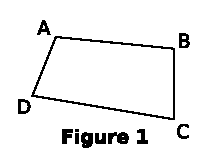
\includegraphics[width=2.8cm]{Q_ABCD}

\vspace{1cm}

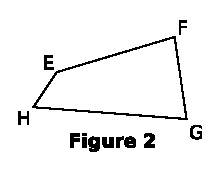
\includegraphics[width=2.8cm]{Q_EFGH}

\vspace{1cm}

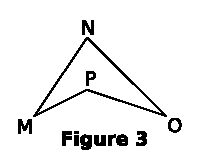
\includegraphics[width=2.6cm]{Q_MNOP}
 \end{minipage} \\

\end{activite}


%%%%%%%%%%%%%%%%%%%%%%%%%%%%%%%%%%%%%%%%%%%%%%%%%%%%%%%%%%%%%%%%%%

\begin{activite}[Une figure à main levée \ldots à l'œil ouvert]
Un professeur demande à ses élèves de tracer les croquis d'un parallélogramme $ABCD$ tel que $AD = 4$ cm, $DC = 7$ cm, $\widehat{ADC} = 72^\circ$. Voici les croquis de cinq élèves : \\[0.5cm]
\begin{tabularx}{0.8\textwidth}{ccccc}
 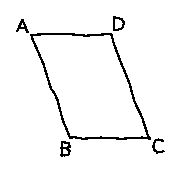
\includegraphics[width=2.3cm]{croquis_1} & 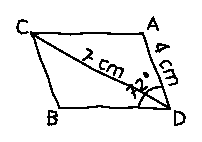
\includegraphics[width=2.7cm]{croquis_2} & 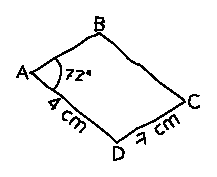
\includegraphics[width=2.8cm]{croquis_3} & 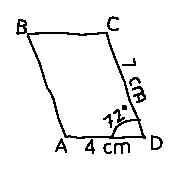
\includegraphics[width=2.3cm]{croquis_4} & 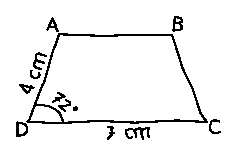
\includegraphics[width=3.1cm]{croquis_5} \\
 Rachid & Élodie & Anissa & Véronique & Patrick \\
\end{tabularx} \\


\begin{enumerate}

\item Qui a fait un croquis correct ? Pour les croquis non corrects, explique l'erreur commise.

\item Construis le parallélogramme $ABCD$.
\end{enumerate}

\end{activite}

%%%%%%%%%%%%%%%%%%%%%%%%%%%%%%%%%%%%%%%%%%%%%%%%%%%%%%%%%%%%%%%%%%

\newpage

\begin{activite}[Puzzle de Sam Lloyd]

\begin{partie}[Construction du puzzle]

\begin{minipage}[c]{0.3\linewidth}
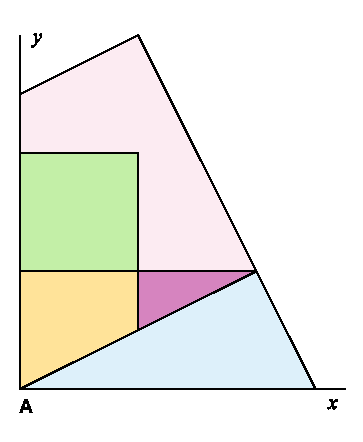
\includegraphics[width=5.2cm]{puzzle}
\end{minipage} \hfill%
\begin{minipage}[c]{0.56\linewidth}
 
  \begin{itemize}
   \item Construis deux demi‑droites perpendiculaires $[Ax)$ et $[Ay)$, puis trace le cercle de centre $A$ et de rayon 7,5 cm. Il coupe $[Ax)$ en $B$ et $[Ay)$ en $C$ ;
   \item Sur $[AC]$, place les points $E$ et $F$ tels que $AE = EF = 3$ cm ;
   \item Trace la perpendiculaire à $(AE)$ passant par $E$ et place les points $G$ et $H$ sur cette droite tels que : $EG = GH = 3$ cm ;
   \item Trace $(BH)$, puis la perpendiculaire à $(BH)$ passant par $C$. Elle coupe $(BH)$ en $J$ ;
   \item Trace $[AH]$ ;
   \item Trace la droite $d_1$ perpendiculaire à $(AE)$ passant par $F$, puis la perpendiculaire à $(EH)$ passant par $G$ qui coupe $[AH]$ en $I$ et $d_1$ en $K$.
   \end{itemize}

\end{minipage} \\

 \end{partie}

Gomme les traits de construction afin de ne conserver que ceux du modèle ci‑dessus.
   
Découpe les cinq pièces du puzzle. 

\begin{partie}[Utilisation du puzzle]
Utilise toutes les pièces du puzzle pour former un carré, un rectangle et un parallélogramme. Construis une solution sur ton cahier pour chacune des formes demandées.
 \end{partie}
 
\end{activite}


\cours
\section{Définitions et propriétés des principaux quadrilatères particuliers}

\begin{definition}
Le \MotDefinition{parallélogramme}{} :

Un quadrilatère dont les côtés opposés sont \textcolor{C2}{\textbf{parallèles deux à deux}} est un parallélogramme. \\[-5em]
\begin{minipage}[t]{0.76\linewidth}
\textcolor{H1}{\textbf{Propriétés}} : dans un parallélogramme :
\begin{itemize}
 \item Les côtés opposés sont \textcolor{H1}{\textbf{parallèles}} et ont \textcolor{H1}{\textbf{la même longueur}} ;
 \item Les diagonales se coupent \textcolor{H1}{\textbf{en leur milieu}} ;
 \item Les angles opposés sont \textcolor{H1}{\textbf{égaux}}.
 \end{itemize}
 \end{minipage}
 \begin{minipage}[c]{0.18\linewidth}
 \vspace{1cm}
  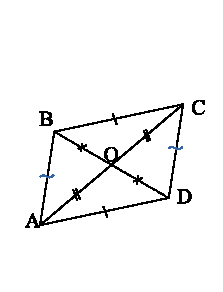
\includegraphics[width=2.5cm]{losangeABCDO}
  \end{minipage} \\
\end{definition}

\begin{minipage}[t]{0.49\linewidth}
\begin{center} 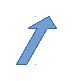
\includegraphics[width=0.8cm]{flash_droite} \end{center}
 \end{minipage}
 \begin{minipage}[t]{0.49\linewidth}
\begin{center} 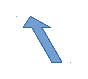
\includegraphics[width=1.1cm]{flash_gauche} \end{center}
 \end{minipage} \\[-2em]

\begin{minipage}[t]{0.49\linewidth}
  \begin{definition}
   Le \MotDefinition{rectangle}{} :
   Un quadrilatère qui a \textcolor{C2}{\textbf{4 angles droits}} est un rectangle.
   
    \begin{center}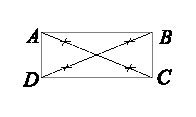
\includegraphics[width=3.5cm]{rectangleABCD}\end{center}
    
   \textcolor{H1}{\textbf{Propriétés}} :
    \begin{itemize}
     \item Un rectangle est un \textcolor{H1}{\textbf{parallélogramme}} donc il possède toutes les propriétés d'un \textcolor{H1}{\textbf{parallélogramme}} ;
     \item Les diagonales d'un rectangle ont \textcolor{H1}{\textbf{la même longueur}}.
     \end{itemize}
   \end{definition}
 \end{minipage}
 %
 \begin{minipage}[t]{0.59\linewidth}
   \begin{definition}
   Le \MotDefinition{losange}{} :
   Un quadrilatère qui a \textcolor{C2}{\textbf{4 côtés de même longueur}} est un losange.
   
     \begin{center}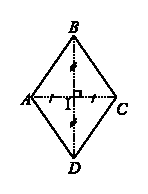
\includegraphics[width=2cm]{losangeABCD2}\end{center}
    
   \textcolor{H1}{\textbf{Propriétés}} :
    \begin{itemize}
     \item Un losange est un \textcolor{H1}{\textbf{parallélogramme}} donc il possède toutes les propriétés d'un \textcolor{H1}{\textbf{parallélogramme}} ;
     \item Les diagonales d'un losange se coupent \textcolor{H1}{\textbf{en leur milieu}} et sont \textcolor{H1}{\textbf{perpendiculaires}}.
     \end{itemize}
   \end{definition}
  \end{minipage} \\
  
\begin{minipage}[t]{0.49\linewidth}
\begin{center} 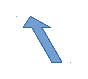
\includegraphics[width=1.1cm]{flash_gauche} \end{center}
 \end{minipage}
 \begin{minipage}[t]{0.49\linewidth}
\begin{center} 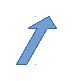
\includegraphics[width=0.8cm]{flash_droite} \end{center}
 \end{minipage} \\ [-2em]
  
\begin{definition}
Le \MotDefinition{carré}{} :

Un quadrilatère qui a \textcolor{C2}{\textbf{4 côtés de même longueur et 4 angles droits}} est un carré. \\[-3em]
\begin{minipage}[t]{0.7\linewidth}
\textcolor{H1}{\textbf{Propriétés}} :
\begin{itemize}
 \item Un carré est à la fois \textcolor{H1}{\textbf{un parallélogramme}}, \textcolor{H1}{\textbf{un losange}} et \textcolor{H1}{\textbf{un rectangle}} donc il a toutes les propriétés de ces quadrilatères ;
 \item Les diagonales d'un carré sont \textcolor{H1}{\textbf{perpendiculaires}} et \textcolor{H1}{\textbf{de même longueur}}.
 \end{itemize}
 \end{minipage}
 \begin{minipage}[c]{0.18\linewidth}
 \vspace{1cm}
 \centering
  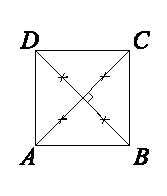
\includegraphics[width=2cm]{carreABCD}
  \end{minipage} \\
\end{definition}



\section{Méthodes de construction}

\begin{methode*1}[Construire un parallélogramme avec la règle et l'équerre]

\vspace{0.8em}
\textcolor{H1}{\textbf{Remarque}} : On utilise ici le fait que les côtés opposés sont parallèles deux à deux.

\begin{exemple*1}
Soient trois points $A$, $B$ et $C$ non alignés. Place le point $D$ tel que $ABCD$ soit un parallélogramme.\\[0.5em]


\begin{tabularx}{\textwidth}{X|X|X}
 \qquad 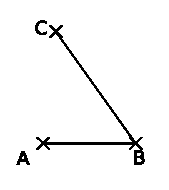
\includegraphics[width=2.1cm]{angleABC8} & 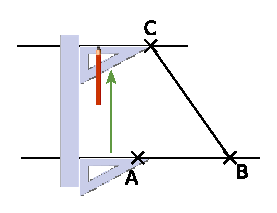
\includegraphics[width=3cm]{angle_parallele} & 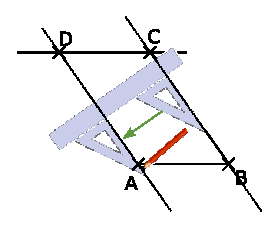
\includegraphics[width=3cm]{quadABCD} \\ 
 On trace les côtés $[AB]$ et $[BC]$ du quadrilatère $ABCD$. Le quadrilatère $ABCD$ est un parallélogramme, donc ses côtés opposés sont parallèles deux à deux : soit $(AB) \parallel (CD)$. & On trace la parallèle à $(AB)$ passant par $C$. & On trace la parallèle à $(BC)$ passant par $A$. Ces deux droites sont sécantes en $D$.
 
 Ainsi $ABCD$ a ses côtés opposés parallèles deux à deux, c'est donc bien un parallélogramme. \\
\end{tabularx} \\[1em]

\end{exemple*1}

\exercice
Réalise un croquis avant de construire le parallélogramme $PRLG$ tel que $PR = 5$ cm, $PG = 6$ cm et  $\widehat{RPG} = 74^\circ$ en utilisant la propriété sur le parallélisme des côtés opposés du parallélogramme.
%\correction

\end{methode*1}

\newpage





\begin{methode*1}[Construire un parallélogramme avec le compas]

 
\vspace{0.8em}
\textcolor{H1}{\textbf{Remarque}} : On utilise ici le fait que les côtés opposés d'un parallélogramme sont égaux deux à deux.

 \begin{exemple*1}
 
  \begin{tabularx}{\textwidth}{X|X|X}
 \qquad 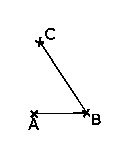
\includegraphics[width=1.2cm]{angleABC_2} & \qquad 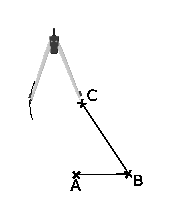
\includegraphics[width=1.9cm]{compasABC} & 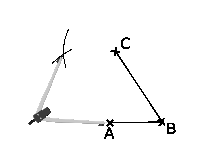
\includegraphics[width=2.4cm]{compasABCD}  \\ 
 On trace les côtés $[AB]$ et $[BC]$ du quadrilatère $ABCD$.
 
 Le quadrilatère $ABCD$ est un parallélogramme, donc ses côtés opposés $[AB]$ et $[CD]$ sont de la même longueur deux à deux : soit $AB = CD$ et $BC = AD$. & À l'aide du compas, on reporte la longueur $AB$ à partir du point $C$. & On reporte la longueur $BC$ à partir du point $A$. On place le point $D$ à l'intersection des deux arcs de cercle puis on trace les côtés $[AD]$ et $[CD]$.
 
Ainsi $ABCD$ a ses côtés opposés égaux deux à deux, c'est donc bien un parallélogramme.\\
\end{tabularx} \\
 
 \end{exemple*1}

\vspace*{1em}
Pour les deux exemples ci-dessous, faire un croquis avant de faire le tracé précis :\\[-2.5em]

\exercice
Construis le parallélogramme $DRAP$ tel que $DR = 6$ cm, $DP = 8$ cm et $\widehat{RDP} = 40^\circ$ en utilisant la propriété sur l'égalité des longueurs des côtés opposés du parallélogramme.
%\correction

\vspace{2.7cm}

\exercice
Construis un rectangle $ABCD$ tel que $AB = 3$ cm et $BC = 5$ cm.
%\correction

\end{methode*1}

%%%%%%%%%%%%%%%%%%%%%%%%%%%%%%%%%%%%%%%%%%%%%%%%%%%%%%%%%%%%

\begin{methode*1}[Construire un losange avec le compas]
 
\vspace{0.8em}
\textcolor{H1}{\textbf{Remarque}} : On utilise ici le fait qu'un losange a quatre côtés de même longueur.

\begin{exemple*1}
Construis un losange $ABCD$ de 6 cm de côté.\\[1em]
\begin{minipage}[c]{0.7\linewidth}
On fait d'abord un croquis. Dans un losange, les quatre côtés ont la même longueur. Ainsi, les triangles $ABD$ et $CBD$ sont \textbf{isocèles} respectivement en $A$ et $C$.
 \end{minipage} \hfill%
 \begin{minipage}[c]{0.24\linewidth}
  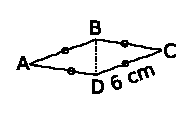
\includegraphics[width=2.6cm]{losange_croquis}
  \end{minipage} \\
  
\begin{tabularx}{\textwidth}{X|X}
 \qquad 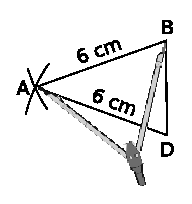
\includegraphics[width=2.6cm]{triangleABD} & 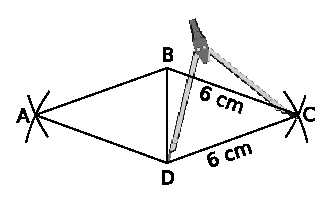
\includegraphics[width=4.8cm]{losangeABCD} \\ 
 On trace un segment $[BD]$. On construit un triangle $ABD$ isocèle en $A$ tel que $AB = AD = 6$ cm. & On construit le triangle $CBD$ isocèle en $C$ tel que $CB = CD = 6$ cm. \\
\end{tabularx} \\

 \end{exemple*1}

\exercice
Construis un losange $VERT$ tel que $VE = 4,5$ cm et $ET = 6,9$ cm.
%\correction

\vspace{3.5cm}

\exercice
Construis un triangle $BOL$ isocèle en $B$ tel que $BO = 2,1$ cm et $OL = 3,4$ cm. Place le point $S$ pour que $BOSL$ soit un losange.
%\correction

\end{methode*1}

%%%%%%%%%%%%%%%%%%%%%%%%%%%%%%%%%%%%%%%%%%%%%%%%%%%%%%%%%%%%



\exercicesbase
\begin{colonne*exercice}

\begin{exercice}[Un peu de vocabulaire]
Recopie et complète les phrases en utilisant les mots « côtés », « sommets », « diagonales », « opposés » et « consécutifs ».\\[-3em]
\begin{minipage}[c]{0.26\linewidth}
\vspace{2cm}
 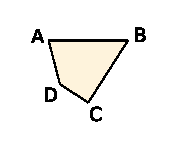
\includegraphics[width=2cm]{quad_rose}
 \end{minipage} \hfill%
 \begin{minipage}[t]{0.66\linewidth}
 Dans le quadrilatère $ABCD$ :
 \begin{enumerate}
  \item $[AB]$ et $[CD]$ sont des \ldots \ldots \ldots ;
  \item $C$ et $D$ sont des \ldots \ldots \ldots ;
  \item $[AD]$ et $[BC]$ sont des \ldots \ldots \ldots ;
  \item $[AC]$ et $[BD]$ sont les \ldots \ldots \ldots ;
  \item $A$ et $C$ sont des \ldots \ldots \ldots ;
  \item $[AB]$ et $[BC]$ sont des \ldots \ldots \ldots .
  \end{enumerate}
 \end{minipage} \\
\end{exercice}

%%%%%%%%%%%%%%%%%%%%%%%%%%%%%%%%%%%%%%%%%%%%%%%%%%%%%%%%%%%%%%%%%

\serie{parallélogrammes}


\begin{exercice}
Construis les parallélogrammes donnés par leur croquis dont les mesures sont données en cm. Dans chacun des cas, précise quelle propriété a été utilisée pour la construction :
\begin{colenumerate}{2}
 \item
 
 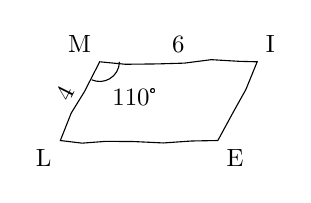
\begin{tikzpicture}[rotate=0,every node/.style={scale=0.9},scale=0.5]

\coordinate (M) at (0,0);
\coordinate (I) at (4,0);
\coordinate (E) at (3,-2);
\coordinate (L) at (-1,-2);

\draw[decorate,decoration={random steps,amplitude=1pt,segment length=10pt}] (M) node [above left]{M}--(I) node [above right]{I}--(E) node [below right] {E}--(L) node [below left] {L}--cycle;

\draw (0.5,0) arc (0:-114:0.5);
\node at (0.9,-0.9){110°};

\path (M)--(L) node[midway,above,sloped]{4};
\path (M)--(I) node[midway,above]{6};
\end{tikzpicture}
  \item
 
 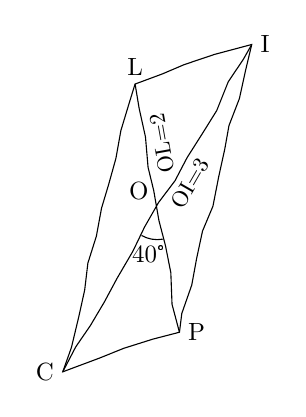
\begin{tikzpicture}[rotate=60,every node/.style={scale=0.9},scale=0.8]

\coordinate (C) at (0,0);
\coordinate (L) at (4.53,1.29);
\coordinate (I) at (6,0);
\coordinate (P) at (1.47,-1.29);
\coordinate (O) at (3,0); %le centre du parallélogramme

\draw[decorate,decoration={random steps,amplitude=1pt,segment length=10pt}] (C) node [left]{C}--(L) node [above]{L}--(I) node [right] {I}--(P) node [right] {P}--cycle;

\draw [decorate,decoration={random steps,amplitude=1pt,segment length=10pt}] (C)--(I) (L)--(P);
\draw (2.5,0) arc (-180:-140:0.5);
\draw (2.3,-0.25) node {40°};
\draw (O) node [above left]{O};

\path (O)--(I) node[pos=0.2,below,sloped,scale=0.9,rotate=60]{OI=3};
\path (O)--(L) node[midway,below,sloped,scale=0.9,rotate=60]{OL=2};

\end{tikzpicture}


  \item
 
 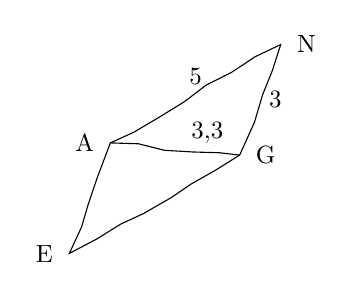
\begin{tikzpicture}[rotate=30,every node/.style={scale=0.9},scale=0.5]

\coordinate (A) at (0,0);
\coordinate (N) at (5,0);
\coordinate (G) at (2.69,-1.91);
\coordinate (E) at (-2.31,-1.91);

\draw[decorate,decoration={random steps,amplitude=1pt,segment length=10pt}] (A) node [left=3pt]{A}--(N) node [right=3pt]{N}--(G) node [right=3pt] {G}--(E) node [left=3pt] {E}--cycle;
\draw [decorate,decoration={random steps,amplitude=1pt,segment length=10pt}] (A)--(G);
\path (A)--(N) node[midway,above]{5};
\path (N)--(G) node[midway,right]{3};
\path (A)--(G) node[near end,above]{3,3};

\end{tikzpicture}
  \item
 
 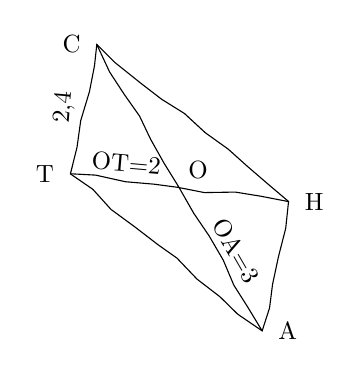
\begin{tikzpicture}[rotate=-60,every node/.style={scale=0.9},scale=0.7]

\coordinate (C) at (0,0);
\coordinate (H) at (4.21,1.59);
\coordinate (A) at (6,0);
\coordinate (T) at (1.79,-1.59);
\coordinate (O) at (3,0); %le centre du parallélogramme

\draw[decorate,decoration={random steps,amplitude=1pt,segment length=10pt}] (C) node [left=3pt]{C}--(H) node [right=3pt]{H} --(A) node [right=3pt] {A}--(T) node [left=3pt] {T}--cycle;
\draw [decorate,decoration={random steps,amplitude=1pt,segment length=10pt}] (C)--(A) (H)--(T);
\node at (O)[above right]{O}; 
\node at (4.5,0)[above,rotate=-60]{OA=3};
\path (C)--(T) node[midway,above,rotate=85]{2,4};
\path (T)--(O) node[midway,above,rotate=-5]{OT=2};

\end{tikzpicture}

 \end{colenumerate}
\end{exercice}


\begin{exercice}
Lorsque c'est possible, construis les parallélogrammes $ABCD$ suivants. Quand la construction n'est pas possible, explique pourquoi :
\begin{enumerate}
 \item $AB = 5$ cm, $AD = 3,5$ cm et $BD = 7$ cm ;
 \item $AB = 2$ cm, $AD = 4,5$ cm et $BD= 3,5$ cm ;
 \item $AD = 4$ cm, $AB = 2,8$ cm et $BD = 7$ cm ;
 \item Construis un carré $IJKL$ tel que $IK = 6,4$ cm.
 \end{enumerate}
\end{exercice}


\begin{exercice}
Pour chacun des parallélogrammes suivants, fais d’abord un croquis puis construis :
\begin{enumerate}
 \item $VERT$ avec $VT = 5$ cm, $\widehat{ERT} = 125^\circ$ et $VE = 4$ cm ;
 \item $BLEU$ de centre $I$ avec $BL = 6$ cm, $UI = 3$ cm et $IE = 4$ cm ;
 \item $NOIR$ avec $NI = 62$ mm, $\widehat{NIR} = 40^\circ$ et $\widehat{RNI} = 30^\circ$.  
 \end{enumerate}
\end{exercice}

\begin{exercice}
Trace un segment $[GR]$ de 7 cm. Construis un parallélogramme dont $[GR]$ est un côté puis un autre dont $[GR]$ est une diagonale.
\end{exercice}


\begin{exercice}[Avec trois points]
\begin{enumerate}
 \item Place trois points $P$, $I$ et $M$ tels que le segment $PI = 4$ cm, le segment $IM = 5$ cm et l'angle $\widehat{PIM} = 130^\circ$ ;
 \item Trouve tous les points $N$ $(N_1, N_2, \ldots)$ tels que les points $P$, $I$, $M$ et $N$ soient les sommets d'un parallélogramme.
 \end{enumerate}
\end{exercice}




%%%%%%%%%%%%%%%%%%%%%%%%%%%%%%%%%%%%%%%%%%%%%%%%%%%%%%%%%%%%%%%%%

\serie{losanges}


\begin{exercice}
Construis les losanges donnés par leur croquis dont les mesures sont données en cm :
\begin{colenumerate}{2}
 \item
 
  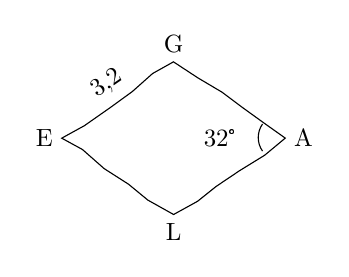
\begin{tikzpicture}[rotate=0,every node/.style={scale=0.9}]

\coordinate (E) at (0,0);
\coordinate (G) at (1.42,0.97);
\coordinate (A) at (2.84,0);
\coordinate (L) at (1.42,-0.97);



\draw[decorate,decoration={random steps,amplitude=1pt,segment length=10pt}] (E) node [left]{E}--(G) node [above]{G}--(A) node [right] {A}--(L) node [below] {L}--cycle;

\draw (2.55,0.18) arc (145:215:0.3) node [midway, left=5pt] {32°};
\path (E)--(G) node[midway,above,sloped]{3,2};
\end{tikzpicture}
  \item
 
 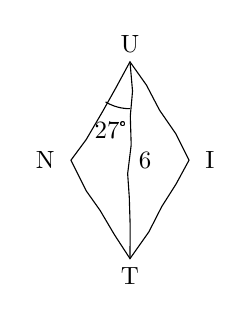
\begin{tikzpicture}[rotate=0,every node/.style={scale=0.9},scale=1]

\coordinate (N) at (0,0);
\coordinate (U) at (0.75,1.25);
\coordinate (I) at (1.5,0);
\coordinate (T) at (0.75,-1.25);

\draw[decorate,decoration={random steps,amplitude=1pt,segment length=10pt}] (N) node [left=3pt]{N}--(U) node [above]{U}--(I) node [right=3pt] {I}--(T) node [below] {T}--cycle;
\draw [decorate,decoration={random steps,amplitude=1pt,segment length=10pt}] (U)--(T);
\path (U)--(T) node[midway,right]{6};
\draw (0.44,0.74) arc (-120.96:-90:0.6) node[near start, below=3pt]{27°};

\end{tikzpicture}
  \item
 
   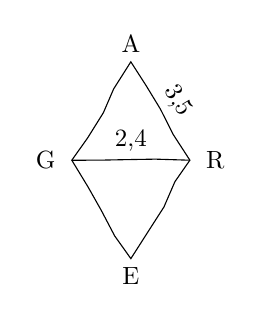
\begin{tikzpicture}[rotate=0,every node/.style={scale=0.9},scale=1]

\coordinate (G) at (0,0);
\coordinate (A) at (0.75,1.25);
\coordinate (R) at (1.5,0);
\coordinate (E) at (0.75,-1.25);

\draw[decorate,decoration={random steps,amplitude=1pt,segment length=10pt}] (G) node [left=3pt]{G}--(A) node [above]{A}--(R) node [right=3pt] {R}--(E) node [below] {E}--cycle;
\draw [decorate,decoration={random steps,amplitude=1pt,segment length=10pt}] (G)--(R);
\path (A)--(R) node[midway,above,sloped]{3,5};
\path (G)--(R) node[midway,above]{2,4};

\end{tikzpicture}
  \item
 
   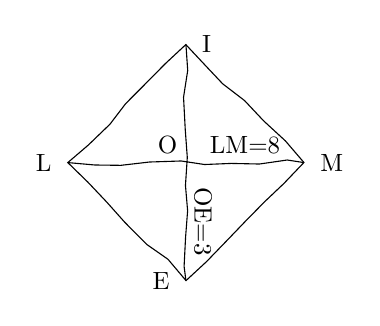
\begin{tikzpicture}[rotate=0,every node/.style={scale=0.9},scale=1]

\coordinate (L) at (0,0);
\coordinate (I) at (1.5,1.5);
\coordinate (M) at (3,0);
\coordinate (E) at (1.5,-1.5);
\coordinate (O) at (1.5,0); %le centre du losange

\draw[decorate,decoration={random steps,amplitude=1pt,segment length=10pt}] (L) node [left=3pt]{L}--(I) node [right=3pt]{I} --(M) node [right=3pt] {M}--(E) node [left=3pt] {E}--cycle;
\draw [decorate,decoration={random steps,amplitude=1pt,segment length=10pt}] (L)--(M) (I)--(E);
\node at (O)[above left]{O}; 
\path (O)--(E) node[midway,above,sloped]{OE=3};
\path (O)--(M) node[midway,above]{LM=8};
\end{tikzpicture}

 \end{colenumerate}
\end{exercice}


\begin{exercice}[Losanges]
\begin{enumerate}
 \item Construis un losange $ABCD$ avec $AB = 4$ cm ; \label{Quadrilateres_entrain}
 \item Sur du papier calque, construis un losange $A'B'C'D'$ tel que $A'B' = 4$ cm et $B'D' = 3,2$ cm.
 
Par superposition, compare cette figure avec celle de la question \ref{Quadrilateres_entrain} ;
 \item Construis un losange $EFGH$ tel que $EF = 32$ mm et $EG = 48$ mm.
 \end{enumerate}
\end{exercice}


\begin{exercice}
Dans chacun des cas suivants, construis un losange $LONG$ tel que :
\begin{enumerate}
 \item $\widehat{OLG} = 31^\circ$ et $LO = 3$ cm ;
 \item $\widehat{LON} = 131^\circ$ et $LO = 3$ cm ;
 \item $\widehat{OLN} = 31^\circ$ et $LO = 3$ cm.
 \end{enumerate}
\end{exercice}


\begin{exercice}[Mon beau losange]
Un professeur demande à trois élèves d'expliquer les différentes étapes pour construire un losange : 
\begin{itemize}
 \item Arnaud dit qu'il trace en pointillés un segment puis fait deux triangles isocèles identiques de chaque côté ;
 \item Sébastien dit qu'il trace en pointillés deux segments perpendiculaires qui se coupent en leur milieu puis qu'il relie leurs extrémités ;
 \item Audrey dit qu'elle trace deux segments de même longueur avec la même extrémité puis qu'elle trace les parallèles à ces deux segments.
 \end{itemize}
 \begin{enumerate}
  \item Pour chaque réponse d'élève, énonce la propriété du losange qui sert à sa construction.
  \item Construis les trois losanges en respectant les programmes de construction de chacun.
 \end{enumerate}
\end{exercice}


%%%%%%%%%%%%%%%%%%%%%%%%%%%%%%%%%%%%%%%%%%%%%%%%%%%%%%%%%%%%%%%%%

\serie{Rectangles}

\begin{exercice}[Des rectangles]
Dans chaque cas, fais d’abord un croquis puis construis :
\begin{enumerate}
 \item $LOUP$ est un rectangle tel que 
 
 $LO = 8$ cm et $LP = 6$ cm ;
 \item $NUIT$ est un rectangle tel que 
 
 $UI = 95$ mm et $IT = 112$ mm.
 \end{enumerate}
\end{exercice}
 
 
\begin{exercice}[D'autres rectangles]
\begin{enumerate}
 \item Construis un rectangle $ABCD$ tel que 
 
 $AB = 7,5$ cm et $AD = 4,8$ cm ;
 \item Construis des points $E$ et $F$ tels que 
 
 $DBEF$ soit un rectangle et $BE = 5$ cm ;
 \item Construis un rectangle $GRIS$ tel que 
 
 $GR = 9$ cm et $GI = 12$ cm ;
 \item Construis un rectangle $LUNE$ tel que 
 
 $LU = 0,6$ dm et $LN = 76$ mm.
 \end{enumerate} 
\end{exercice}


\begin{exercice}
Construis les rectangles donnés par leur croquis dont les mesures sont données en cm :
\begin{colenumerate}{2}
 \item
 
  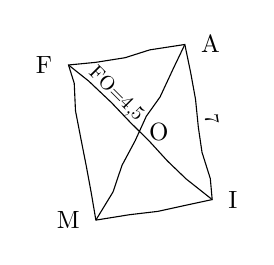
\begin{tikzpicture}[rotate=10,every node/.style={scale=0.9},scale=1]

\coordinate (F) at (0,0);
\coordinate (A) at (1.5,0);
\coordinate (I) at (1.5,-2);
\coordinate (M) at (0,-2);
\coordinate (O) at (0.75,-1); %le centre du rectangle

\draw[decorate,decoration={random steps,amplitude=1pt,segment length=10pt}] (F) node [left=3pt]{F}--(A) node [right=3pt]{A} --(I) node [right=3pt] {I}--(M) node [left=3pt] {M}--cycle;
\draw [decorate,decoration={random steps,amplitude=1pt,segment length=10pt}] (F)--(I) (A)--(M);
\node at (O)[right]{O}; 
\node at (.53,-.47)[rotate=-45,scale=0.8]{FO=4,5};
\path (A)--(I) node[midway,above,rotate=-80,scale=0.8]{7};
%\path (T)--(O) node[midway,above,rotate=-5]{OT=2};

\end{tikzpicture}

  \item
 
   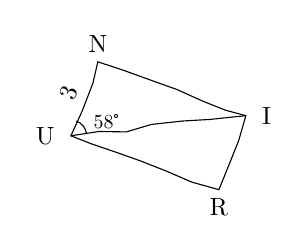
\begin{tikzpicture}[rotate=-20,every node/.style={scale=0.9},scale=1]

\coordinate (U) at (0,0);
\coordinate (N) at (0,1);
\coordinate (I) at (2,1);
\coordinate (R) at (2,0);

\draw[decorate,decoration={random steps,amplitude=1pt,segment length=10pt}] (U) node [left=3pt]{U}--(N) node [above]{N}--(I) node [right=3pt] {I}--(R) node [below] {R}--cycle;
\draw [decorate,decoration={random steps,amplitude=1pt,segment length=10pt}] (U)--(I);
\path (U)--(N) node[midway,above,rotate=70]{3};
\draw (0,0.2) arc (90:26.57:0.2) node[above=5pt,right,scale=0.8]{58°};

\end{tikzpicture}
  \item
 
   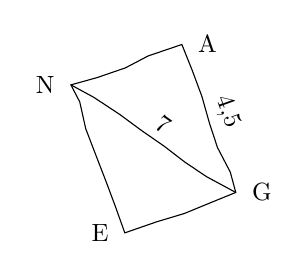
\begin{tikzpicture}[rotate=20,every node/.style={scale=0.9},scale=1]

\coordinate (N) at (0,0);
\coordinate (A) at (1.5,0);
\coordinate (G) at (1.5,-2);
\coordinate (E) at (0,-2);
\coordinate (O) at (0.75,-1); %le centre du rectangle

\draw[decorate,decoration={random steps,amplitude=1pt,segment length=10pt}] (N) node [left=3pt]{N}--(A) node [right=3pt]{A} --(G) node [right=3pt] {G}--(E) node [left=3pt] {E}--cycle;
\draw [decorate,decoration={random steps,amplitude=1pt,segment length=10pt}] (N)--(G);
\node at (.75,-1)[above,rotate=-35]{7};
\path (A)--(G) node[midway,above,rotate=-70]{4,5};

\end{tikzpicture}

  \item
 
   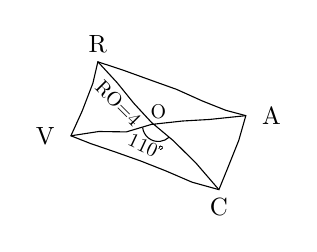
\begin{tikzpicture}[rotate=-20,every node/.style={scale=0.9},scale=1]

\coordinate (V) at (0,0);
\coordinate (R) at (0,1);
\coordinate (A) at (2,1);
\coordinate (C) at (2,0);
\coordinate (O) at (1,0.5);

\draw[decorate,decoration={random steps,amplitude=1pt,segment length=10pt}] (V) node [left=3pt]{V}--(R) node [above]{R}--(A) node [right=3pt] {A}--(C) node [below] {C}--cycle;
\draw [decorate,decoration={random steps,amplitude=1pt,segment length=10pt}] (V)--(A) (R)--(C);

\path (R)--(O) node[midway,below,rotate=-45,scale=0.8]{RO=4};
\node[above,scale=0.8] at (O){O};

\draw (0.82,0.41) arc (-153.43:-26.56:0.2) node[below=8pt,left,scale=0.8,rotate=-25]{110°};

\end{tikzpicture}
 \end{colenumerate}
\end{exercice}




%%%%%%%%%%%%%%%%%%%%%%%%%%%%%%%%%%%%%%%%%%%%%%%%%%%%%%%%%%%%%%%%%

\serie{carrés}


\begin{exercice}[Des carrés]
Construis les carrés donnés :
\begin{enumerate}
 \item un carré $BLEU$ de côtés 4 cm ;
 \item carré $LUNA$ de côtés 6,2 cm ;
 \item un carré $IJKL$ tel que $IK = 6,4$ cm.
 \end{enumerate} 
\end{exercice}


\begin{exercice}[Programme de construction]
Écris un programme de construction pour la figure suivante :

\begin{minipage}[c]{0.46\linewidth}
$d' \parallel (OM)$

$LM = MN = 5$ cm
 \end{minipage} \hfill%
 \begin{minipage}[c]{0.46\linewidth}
  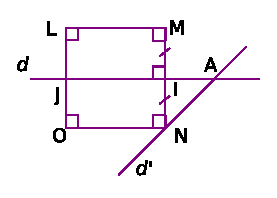
\includegraphics[width=4cm]{programme2}
  \end{minipage} \\
\end{exercice}


\begin{exercice}
Trace une droite $d$ et place un point $R$ qui n'appartient pas à $d$ ;

Construis un carré de sommet $R$, ayant pour axe de symétrie la droite $d$. Combien y a‑t‑il de solutions ?

\end{exercice}


%%%%%%%%%%%%%%%%%%%%%%%%%%%%%%%%%%%%%%%%%%%%%%%%%%%%%%%%%%%%%%%%%

\serie{quadrilatères mélangés…}

\begin{exercice}[Reconnaître]
Quelle est la nature de chaque quadrilatère $ABCD$ :
\begin{center} 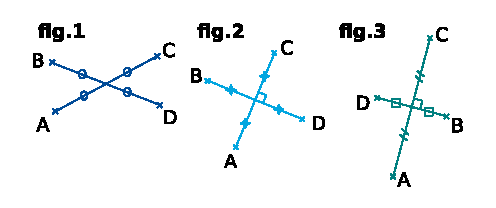
\includegraphics[width=6.8cm]{quadABCD2} \end{center}
\end{exercice}


\begin{exercice}[Constructions]
Construis le rectangle $MODE$ et le losange $CHUT$ :

\qquad 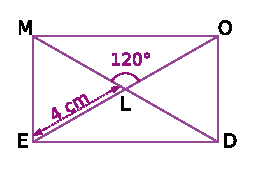
\includegraphics[width=3.4cm]{quadDEMO} \qquad 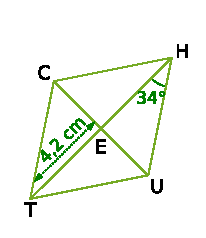
\includegraphics[width=2.5cm]{quadCHTU}
\end{exercice}



\begin{exercice}
Pour chacun des quadrilatères suivants, fais d’abord un croquis puis construis :
\begin{enumerate}
 \item Le rectangle $MANU$ tel que 
 
 $MN = 9$ cm et $MA = 5$ cm ;
 \item Le losange $OURS$ tel que 
 
 $OR = 8$ cm et $US = 6$ cm ;
 \item Le rectangle $PAUL$ tel que 
 
 $PA = 8$ cm et $\widehat{LAU} = 53^\circ$. 
 
 Rédige le programme de construction correspondant.
 \end{enumerate}
\end{exercice}


\begin{exercice}[Une enveloppe plus grande]
\vspace{1em}
\begin{minipage}[c]{0.50\linewidth}
Construis une figure trois fois plus grande en utilisant uniquement ta règle non graduée et ton compas.
 \end{minipage} \hfill%
 \begin{minipage}[c]{0.42\linewidth}
  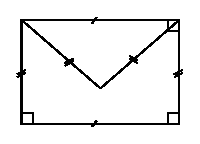
\includegraphics[width=2.6cm]{enveloppe}
  \end{minipage} \\
\end{exercice}


%%%%%%%%%%%%%%%%%%%%%%%%%%%%%%%%%%%%%%%%%%%%%%%%%%%%%%%%%%%%%%%%%
\vspace{1em}
\serie{cercles}

\begin{exercice}[Deux droites sécantes et un cercle]
 \begin{enumerate}
  \item Trace deux droites $d$ et $d'$ sécantes en $O$ sans qu'elles soient perpendiculaires. Place un point $A$ sur $d$. Trace le cercle de centre $O$ et de rayon $OA$. Il recoupe $d$ en $A'$ et $d'$ en $B$ et $B'$ ;
  \item Quelle semble être la nature du quadrilatère $ABA'B'$ ? Et si $d$ et $d'$ sont perpendiculaires ?
  \end{enumerate}
\end{exercice}


\begin{exercice}[Avec des cercles]
\vspace{1em}
Trace deux cercles concentriques de centre $O$. En te servant uniquement d'une règle non graduée, trace un parallélogramme de centre $O$ dont deux sommets appartiennent à l'un des cercles et les deux autres à l'autre cercle.
\end{exercice}



\end{colonne*exercice}


\exercicesappr
\begin{colonne*exercice}
\begin{exercice}[Renard rusé]
Un poulailler grillagé de forme rectangulaire mesure 10 mètres de long et 6 mètres de large. Médor, le premier chien de garde, est attaché à un piquet à l'angle du poulailler avec une chaîne de 15 mètres. Il doit surveiller le grillage mais ne peut pas rentrer dans l'enclos. 
\begin{enumerate}
 \item Dessine le poulailler, en précisant l'échelle appropriée que tu auras choisie, puis colorie en rouge la zone protégée par Médor. Repasse en noir la partie du grillage que le renard pourrait attaquer sans danger.
 \item Barbac, le second chien de garde est attaché avec une chaîne de 10 mètres, à l'angle du poulailler le plus proche de celui de Médor.
 
Sur le même schéma, colorie en bleu la zone protégée par Barbac. Le renard peut-il encore attaquer le grillage du poulailler en toute sécurité ?
 \end{enumerate}
\end{exercice}


\begin{exercice}[Agrandissement]
Reproduis la figure en doublant ses dimensions.
\begin{center} 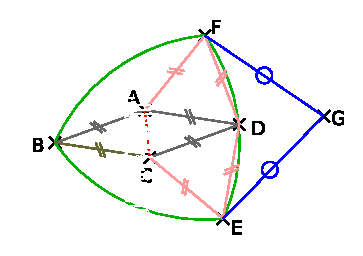
\includegraphics[width=5cm]{agrandissement} \end{center}
\end{exercice}


\begin{exercice}[Construction de l'hexagone]

\vspace{1em}

\begin{minipage}[c]{0.50\linewidth}
Observe attentivement le codage de la figure ci‑contre. 

Déduis-en une méthode pour construire un hexagone régulier de 4 cm de côté puis effectue la construction sur ton cahier.
 \end{minipage} \hfill%
 \begin{minipage}[c]{0.46\linewidth}
  \begin{center} 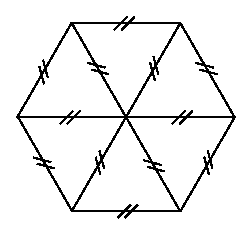
\includegraphics[width=3.5cm]{hexagone} \end{center}
  \end{minipage} \\
\end{exercice}


\begin{exercice}[Quadrilatères inscrits dans un cercle]
\begin{enumerate}
 \item Trace un cercle de centre $O$ et de rayon 5 cm. Trace deux diamètres perpendiculaires qui coupent le cercle en quatre points formant le quadrilatère $RIEN$. Quelle est sa nature ?
 \item Construis les médiatrices de $[NO]$ et de $[OI]$. Elles coupent le cercle en quatre points formant le quadrilatère $TOUS$. Quelle est sa nature ?
 \item Les médiatrices coupent $[NI]$ en deux points $M$ et $A$. Quelle est la nature de $ARME$ ?
 \end{enumerate}
\end{exercice}


\begin{exercice}[Élève absent]
Tu étais absent au dernier cours de mathématiques. Marcel et Célestine se sont partagé le travail pour décrire à leur manière les figures. Reproduis-les proprement sur ton cahier :
\begin{enumerate}
 \item Marcel te donne le croquis de la première figure intitulée « les lunules d'Hippocrate ».
 \begin{center} 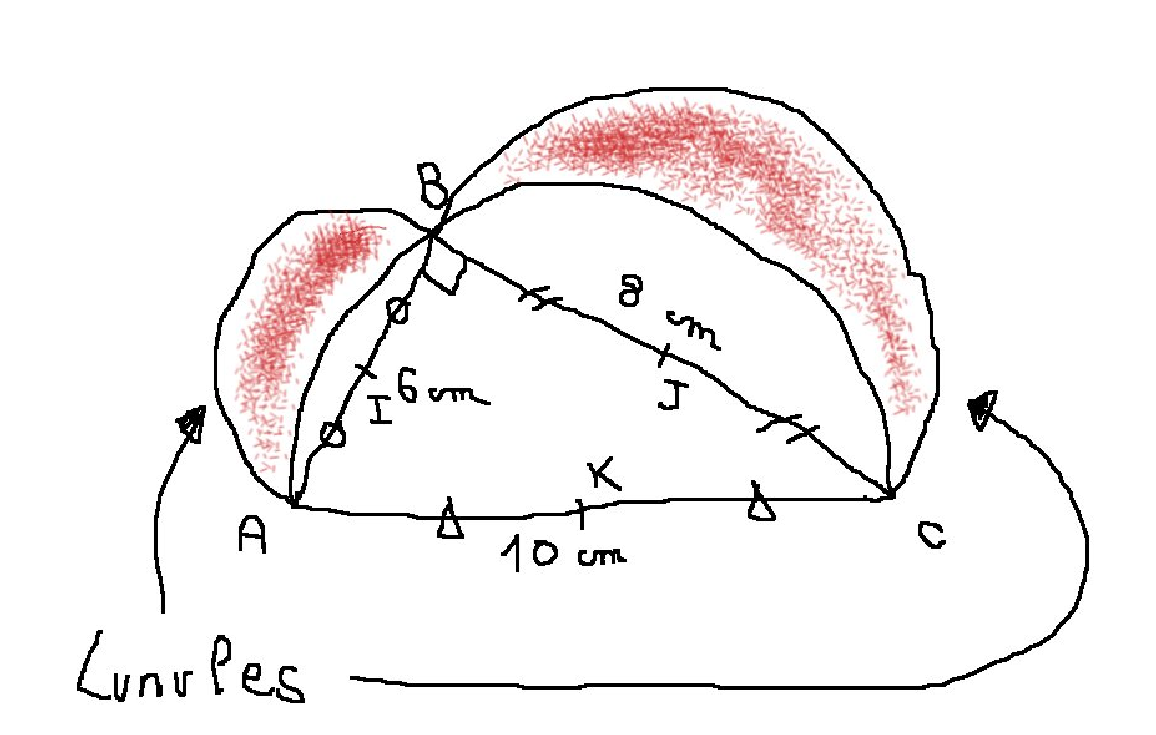
\includegraphics[width=6.8cm]{lunules} \end{center}
 \item Célestine te donne un programme de construction d'un carré $ABCD$ à la règle et au compas :
 
« D'abord, tu traces deux points $A$ et $B$, et la droite $(AB)$.

Pour tracer la droite perpendiculaire à $(AB)$ passant par $A$, tu fais comme cela :
 \begin{itemize}
  \item Place un point $K$ de manière à ce que $A$ soit le milieu de $[KB]$ ;
  \item Trouve un point $L$, équidistant de $K$ et de $B$, autre que le milieu $A$ ;
  \item Trace la droite $(AL)$.
  \end{itemize}
Ensuite, tu fais de la même manière pour tracer la perpendiculaire à $(AB)$ passant par $B$.
  
Enfin, comme tu sais que les côtés d'un carré ont tous la même longueur, tu trouves les points $C$ et $D$.

Et puis pour finir, tu traces joliment ton carré au stylo … »

 \end{enumerate}
\end{exercice}


%%%%%%%%%%%%%%%%%%%%%%%%%%Mise en page

\vspace*{1cm}

\phantom{Pour sauter une ligne}

\newpage
%%%%%%%%%%%%%%%%%%%%%%%%%%%%%%%%%%%%%%




\begin{exercice}[Un intrus]
Construis les figures données par les trois programmes. Quelle est la figure différente des deux autres ?

\begin{enumerate}
 \item \textbf{Programme 1}
 
Trace un cercle de diamètre $[CD]$, de centre $O$ et de rayon 3 cm ;

Place le point $B$ tel que $C$ soit le milieu de $[BO]$ ;

Construis le triangle $ABC$ tel que $AB = 4$ cm et $AC = 5$ cm ;

Trace le segment $[AD]$ ;

Trace les cercles de diamètre $[AD]$ et $[AC]$.

 \item \textbf{Programme 2}
 
Trace un segment $[AC]$ de longueur 5 cm, puis trace le cercle de diamètre $[AC]$ ;

Place un point $B$ sur ce cercle à 4 cm du point $A$ et trace les segments $[AB]$ et $[BC]$ ;

Place les points $O$ et $D$ de manière à ce que les points $B$, $C$, $O$ et $D$ soient alignés dans cet ordre et régulièrement espacés ;

Trace le segment $[AD]$, le cercle de diamètre $[AD]$ et le cercle de centre $O$ passant par $D$.
 \item \textbf{Programme 3}
 
Trace un segment $[AD]$ de longueur 13 cm, et le cercle de diamètre $[AD]$ ;

Place un point $B$ sur le cercle précédent et à 5 cm de $A$ ;

Trace le segment $[BD]$ ;

Place le point $O$ sur le segment $[BD]$ à 4 cm du point $D$ ;

Trace le cercle de centre $O$ passant par $D$, il coupe le segment $[BD]$ en $C$ ;

Trace le segment $[AC]$ ;

Trace le cercle de diamètre $[AC]$.
 \end{enumerate}
\end{exercice}

\end{colonne*exercice}

\connaissances

\QCMautoevaluation{Pour chaque question, plusieurs réponses sont
  proposées.  Déterminer celles qui sont correctes.}

\begin{QCM}
  \begin{GroupeQCM}
    \begin{exercice}
      Si $T$ est le milieu d'un segment $[AD]$ et que $AD = 56$ mm alors \ldots
      \begin{ChoixQCM}{4}
      \item $T \in [AD]$
      
      et $TA = 28$ mm
      \item $TA = TD$
      \item \\[-1em]
      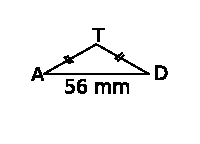
\includegraphics[width=2.6cm]{triangleATD}
      \item $[AD]$ est un diamètre du cercle de centre $T$ et de rayon 28 mm
      \end{ChoixQCM}
\begin{corrige}
     \reponseQCM{abd} 
   \end{corrige}
    \end{exercice}

  \begin{exercice}
      Si $ROSE$ est un losange alors \ldots
      \begin{ChoixQCM}{4}
      \item $[RE]$ est une diagonale
      \item $[OS]$ est une diagonale
      \item $[OS]$ est un côté
      \item $[RS]$ est une diagonale
      \end{ChoixQCM}
\begin{corrige}
     \reponseQCM{cd}
   \end{corrige}
    \end{exercice}


\end{GroupeQCM}
\end{QCM}

  


\TravauxPratiques % pour nous "travailler en groupe"

\begin{TP}[Fractale]

\partie{Dans la cour}

Chaque groupe possède une ficelle de 1 mètre de long, une équerre et des craies de couleur.\\[0.5em]
Le but est de reproduire sur le sol de la cour la figure ci‑dessous, constituée de carrés inscrits les uns dans les autres. \\[0.5em]
Le plus grand carré mesure 1 m de côté.\\[0.5em]
Chaque carré a ses sommets positionnés au tiers de la longueur des côtés du carré précédent.\\[0.5em]
Continuez la construction en variant les couleurs pour chaque carré inscrit.\\[0.5em]
\begin{center} 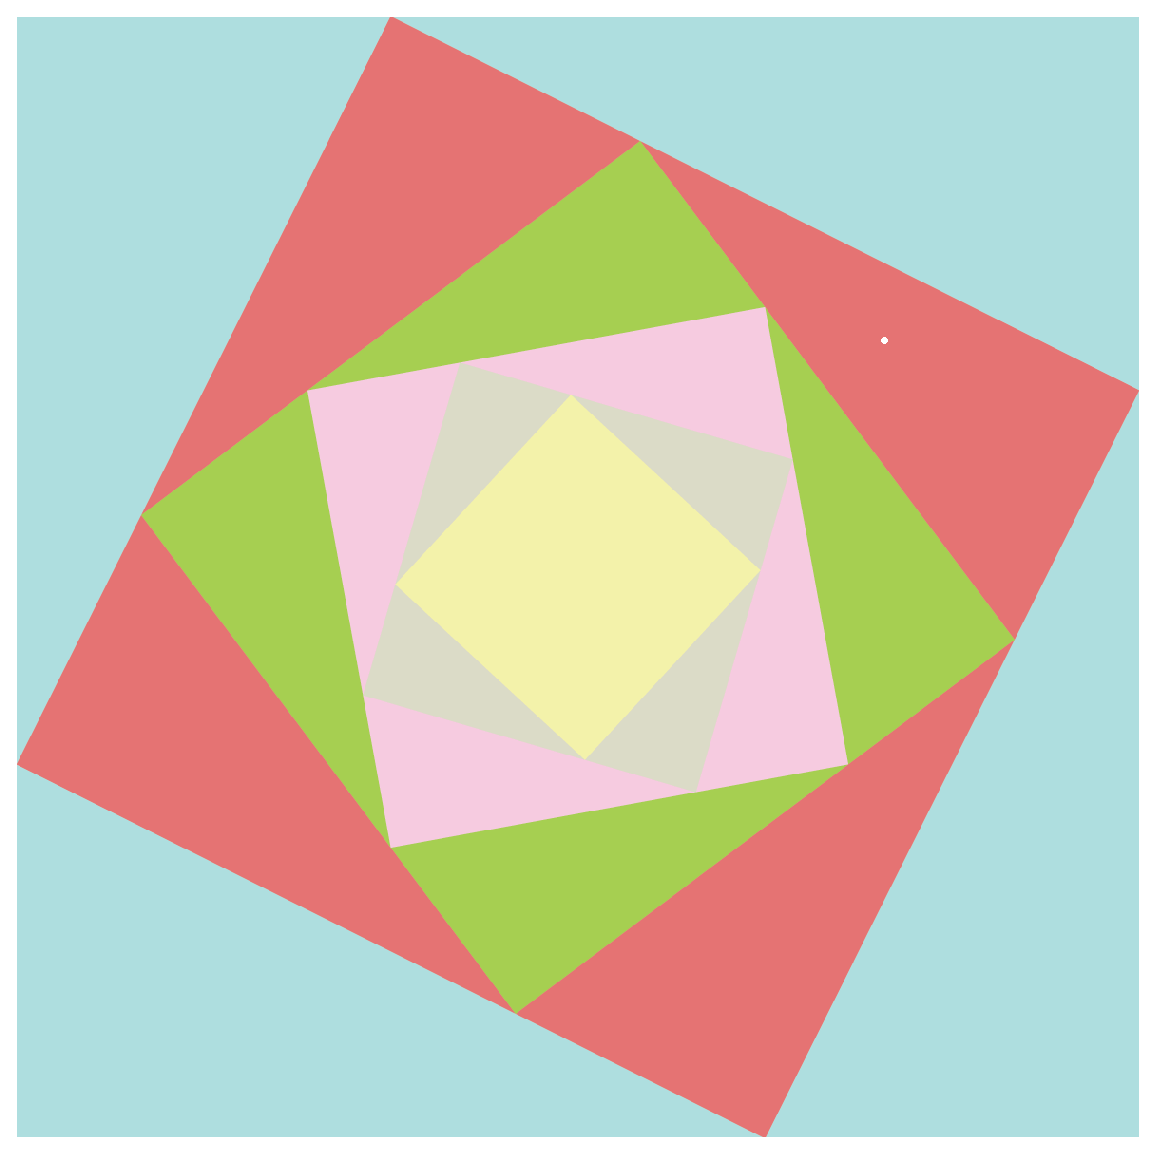
\includegraphics[width=5cm]{fractale} \end{center}

\partie{Sur ton cahier}

Sur ton cahier, reproduis la construction de la figure fractale du carré.\\[0.5em]
Selon la même méthode, dessine ensuite une figure fractale d'un losange.

\end{TP}

%%%%%%%%%%%%%%%%%%%%%%%%%%%%%%%%%%%%%%%%%%%%%%%%%%%%%%%%%%%%%%%%

\begin{TP}[Figures téléphonées]

\partie{Construction de la figure}
Chaque élève construit une figure contenant : cinq points, un cercle ayant son rayon ou son diamètre décrit par deux de ces cinq points, un losange. Le reste de la construction est libre.

\partie{Écriture du programme de construction}
Écris un programme de construction de ta propre figure, en indiquant les longueurs utiles et en nommant les points si nécessaire. Donne ensuite ce programme à ton binôme et conserve la figure initiale cachée.

\partie{Reconstruction de la figure}
Essaie de suivre les instructions du programme que tu as reçu et reproduis le plus fidèlement possible la figure de ton camarade.

Une fois les constructions terminées, valide la construction en comparant la figure construite avec l'originale.

\end{TP}

\newpage


\pagebreak

\recreation
\begin{enigme}[Vitraux de cathédrales]

Dans les deux cas construis un carré de côté 6 cm :

\begin{minipage}[c]{0.3\linewidth}
\end{minipage}\hfill %
\begin{minipage}[c]{0.2\linewidth}
\centering
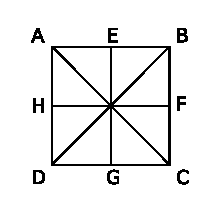
\includegraphics[width=2.8cm]{vitre}
\end{minipage} \hfill %
\begin{minipage}[c]{0.2\linewidth}
\centering
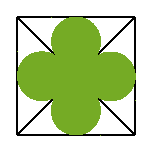
\includegraphics[width=1.9cm]{rosace}
\end{minipage} \hfill %
\begin{minipage}[c]{0.3\linewidth}
\end{minipage} 


\underline{Programme de construction} :
\begin{itemize}
 \item Construis un arc de cercle de centre A et de rayon AE ; il coupe [AC] en un point que tu nommeras I ;
 \item Construis le point J tel que le quadrilatère AEJI soit un losange ;
 \item Nomme K le point d'intersection de la diagonale [AJ] et du segment [EG].
                
Trace le cercle de centre K passant par E ;
 \item Place les points L et N sur le segment [HF] tel que LF = EK = HN ;
 \item Trace le cercle de centre L passant par F et celui de centre N passant par H ;
 \item Place le point M sur le segment [EG] tel que MG = EK ;
 \item Trace le cercle de centre M passant par G.
 \end{itemize}
Tu obtiens ainsi une rosace à quatre branches que tu peux voir dans certaines églises.
 
 \end{enigme}
 
 \vspace*{2em}
 
%%%%%%%%%%%%%%%%%%%%%%%%%%%%%%%%%%%%%%%%%%%%%%%%%%%%%%%%%%%%%%%%%%%%%

\begin{enigme}[L'art de l'islam]

\begin{center}
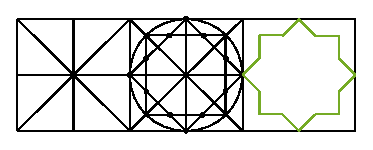
\includegraphics[width=5.4cm]{islam}
\end{center}

Tu peux réaliser une belle frise avec ce motif.
\end{enigme} 



